\documentclass{article}
\usepackage{polski}
\usepackage[utf8]{inputenc}
\title{Wstęp do robotyki - sprawozdanie z laboratorium}
\author{Marta Pacuszka}
\usepackage{graphicx}
\begin{document}
\pagenumbering{gobble}
\maketitle
\newpage
\pagenumbering{arabic}
\section{Opis projektu}
Celem projektu była budowa robota śledzącego linię przy użyciu zestawu klocków Lego Mindstorms EV3, a następnie jego zaprogramowanie tak, aby robot odnalazł na planszy zielony kafelek, podniósł znajdujący się na nim koszyczek i przetransportował go na czerwony kafelek.
\section{Opis budowy robota}
W ramach projektu powstał robot "Zbyszek", przedstawiony na rysunku \ref{zbyszek}. 
\begin{figure}[h]
\centering
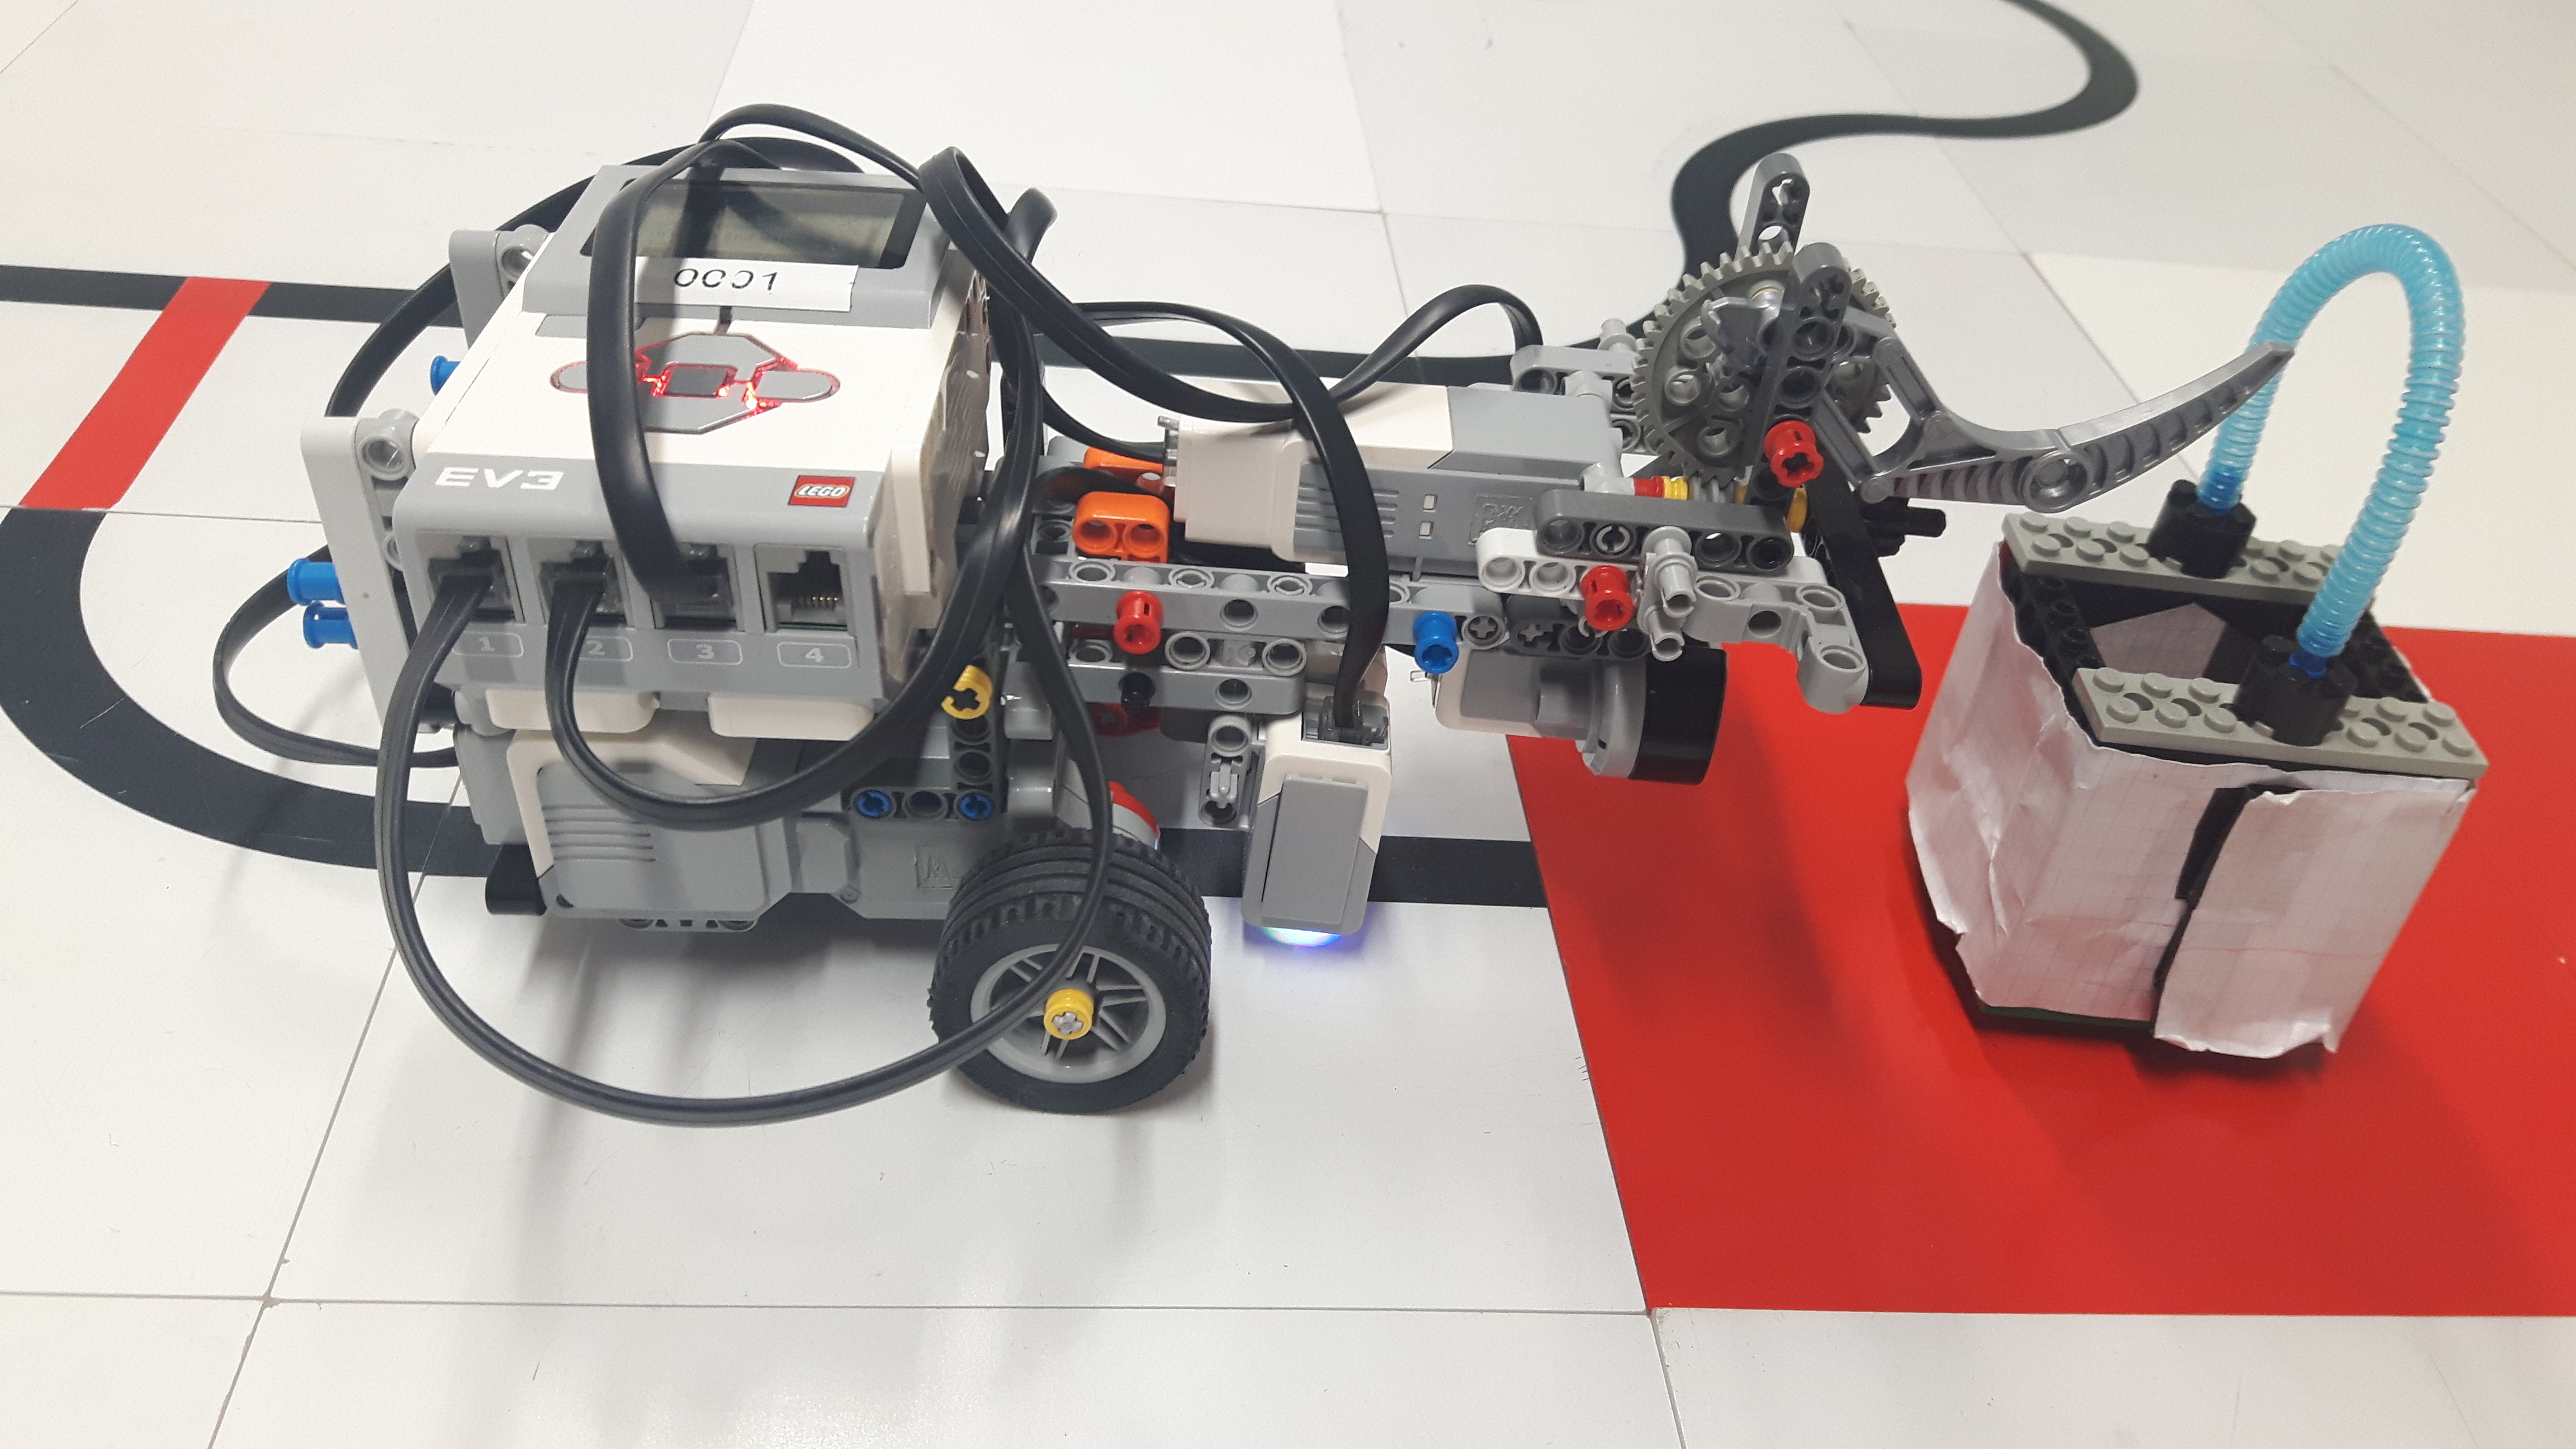
\includegraphics[width=0.5\textwidth]{zbyszek.jpg}
\caption{Robot Zbyszek}
\label{zbyszek}
\end{figure}
Głownym elementem konstrukcyjnym robota jest kostka EV3 - sterownik z systemem Linux. Robot posiada dwa koła sterowane przez dwa duże serwomechanizmy oraz jedno koło wleczone
\paragraph{Czujniki}
\paragraph{Efektory}
\paragraph{Konfiguracja}
\section{Charakterystyka algorytmu podążania za linią}
\subsection{Sposób dobierania parametrów algorytmu}
\subsection{Zalety i wady zastosowanego rozwiązania}
\section{Opis implementacji algorytmów (schemat blokowy)}


\end{document}